\chapter{Hybrid Set Theory}


%%%%%%%%%%%%%%%%%%%%%%%%%%%%%%%%%%%%%%%%%
%
% PIECEWISE
%
%%%%%%%%%%%%%%%%%%%%%%%%%%%%%%%%%%%%%%%%%


The motivation behind hybrid sets and functions can be traced to wanting a better approach to piecewise functions.
Piecewise functions are enormously useful constructions in many areas (...)
The perennial example of a piecewise function is $\mathrm{abs}:\mathbb{R} \to \mathbb{R}_{+} \cup \{ 0 \}$ given in the form:
\begin{equation}
	\mathrm{abs}(x) = 
  		\left\{
     			\begin{array}{lr}
       			-x & : x < 0 \\
       			x & : x \geq 0
     			\end{array}
   		\right.
\end{equation}


To evaluate abs for an argument $x$, one must first determine which sub-function to use. 
If $x < 0$ then the first case is evaluated and abs will return the result of $x \mapsto -x$. 
Otherwise, if $x \geq 0$ the second case is evaluated and the result of $x \mapsto x$ is returned. 
Rather than as a condition, we could just as easily think of ``$x<0$'' and ``$x \geq 0$'' as partitions of the real line.
Evaluation then occurs by checking whether $x\in \mathbb{R}_{+} \cup \{ 0 \} $ or $x \in \mathbb{R}_{-}$.
In general, a piecewise function $f$ will take the form:
\begin{equation}
\label{eq_fP}
	f(x) = 
	  \left\{
	     \begin{array}{lr}
	       f_1(x) & : x \in P_1 \\
	       f_2(x) & : x \in P_2 \\ 
	       \vdots & \vdots \\
	       f_n(x) & : x \in P_n
	     \end{array}
	   \right.
\end{equation}
where the set $\{ P _ i \}$ forms a partition of the domain of $f$ and for each $f_i$ is defined over all of the corresponding $P_i$. To formalize this we require the ability to restrict a function's domain and join disjoint pieces together.


\begin{definition}
	Given a function $f:X \to Y$ for any subset of the domain, 
	$Z \subset X$, the \emph{restriction of $f$ to $Z$} is the function $f|_Z : Z \to Y$, 
	such that $f|_Z(x) = f(x)$ for all $x \in Z$.
\end{definition}


\begin{definition}
	Define $\fjoin$, the \emph{join} of two functions, $f$ and $g$ by:
	\begin{equation}
	\label{def:fjoin}
		f \fjoin g =  
		\left\{
	     		\begin{array}{lr}
	       		f(x) & \text{if } g(x) = \bot \\
	       		g(x) & \text{if } f(x) = \bot \\
	       		\bot & otherwise
	     		\end{array}
	   	\right.
	\end{equation}
\end{definition}


This allows us to re-write our previous definition of (\ref{eq_fP}) as:
\begin{equation}
	\label{fjoin_partition}
	f = \restrict{f}{P_1} \fjoin \restrict{f}{P_2} \fjoin \ldots \fjoin \restrict{f}{P_n}
\end{equation}
But we must be careful as this definition is not associative.
Given functions $f,g,h$ each restricted to the sets $A,B,C$. 
Then for any element in the intersection $x \in A \cap B \cap C$:
\begin{equation}
	( (\restrict{f}{A} \fjoin \restrict{g}{B} ) \fjoin \restrict{h}{C} )(x) = h(x)
\end{equation}
But by rearranging the parentheses we find,
\begin{equation}
	( \restrict{f}{A} \fjoin ( \restrict{g}{B} \fjoin \restrict{h}{C} ))(x) = f(x)
\end{equation}
Other conventions exist, for example \emph{Maple}'s 
\texttt{piecewise(cond\_1, f\_1, cond\_2, f\_2,} \linebreak
\texttt{\ldots, cond\_n, f\_n, f\_otherwise)} 
effectively uses a short-circuted $\fjoin$.
Each of the conditionals, \texttt{cond\_i} are evaluated in order and when one evaluates to true, the corresponding \texttt{f\_i} is evaluted.
Finally if all of \texttt{cond\_i} evaluate to false then \texttt{f\_otherwise} is used.
This approach simply trades associativity for commutivity.


More importantly, when dealing with multiple piecewise functions, expressions cannot be easily simplified without an explosion in terms.
For example, given $f,g$ two piecewise functions 
$f = \left(\restrict{f_1}{P_1} \fjoin \restrict{f_2}{P_2} \fjoin \restrict{f_3}{P_3} \right)$ 
and $g= \left( \restrict{g_1}{Q_1} \fjoin \restrict{g_2}{Q_2} \right)$ their sum $(f+g)$ is:
\begin{align}
	(f+g) = \;
	&\restrict{(f_1+g_1)}{P_1 \cap Q_1} 
		\;\fjoin\; \restrict{(f_1+g_2)}{P_1 \cap Q_2} 
		\;\fjoin\; \restrict{(f_1+g_3)}{P_1 \cap Q_3}\notag\\
	&\restrict{(f_2+g_1)}{P_2 \cap Q_1} 
	 	\;\fjoin\; \restrict{(f_2+g_2)}{P_2 \cap Q_2} 
	 	\;\fjoin\; \restrict{(f_2+g_3)}{P_2 \cap Q_3}
\end{align}
That is, we first create a common refinement by the pairwise intersection of each $P_i$ with each $Q_j$.
Over each intersection we then take the sum of the respective sub-functions.
In general, assuming no degenerate intersections, the sum of an $n$ piece function and $m$ piece function will give a piecewise function with $n\times m$ pieces.
To flatten an expression containing multiple piecewise functions we can very quickly find ourselves with an unreasonable number of pieces.
If we abandon boolean sets, we can construct common refinements much more efficiently as will be shown.





%%%%%%%%%%%%%%%%%%%%%%%%%%%%%%%%%%%%%%%%%
%
% HYBRID SET
%
%%%%%%%%%%%%%%%%%%%%%%%%%%%%%%%%%%%%%%%%%
\section{Hybrid Sets}


We shall consider \emph{hybrid sets}.
One can define traditional sets by an indicator function which maps each member element to 1 and each non member to 0.
A \emph{multiset} or \emph{bag} extends this by allowing multiple copies of the same element.
The indicator function of a multiset would therefore range over $\mathbb{N}_0$, the set of non-negative integers.
For example the types of coins in a currency might be represented as a set: $\{ \$0.01, \$0.05, \$0.10, \$0.25, \$1.00 \}$.
A multiset might represent the physical coins in my pocket: $2 \times \$0.05, 5 \times \$0.10, 1 \times \$1.00$.
Hybrid sets take this one step further allowing for an element to occur \emph{negatively many} times.


\begin{definition}
	Let $U$ be a universe, then any function $U \to \mathbb{Z}$ is called a \textbf{hybrid set}.
\end{definition}


By universe, we just mean a (traditional) set that \emph{contains everything we may be interested in}.
The size of a universe is context dependant but we will rarely be interested in everything in the universe or its exact size.
It is simply a compact way for us to talk about ``everything else''.
This definition of hybrid sets does little good on its own; much of the usefulness of sets is derived from their rich notation.
So with that said,


\begin{definition}
	Let $H$ be a hybrid set. 
	Then we say that $H(x)$ is the \textbf{multiplicity} of the element $x$. 
	We write, $x \in^n H$ if $H(x)=n$. 
	Furthermore we will use $x \in H$ to denote $H(x)\neq 0$ (or equivalently, $x \in^n H$ for $n\neq 0$).
	Conversely, $x \notin H$ denotes $x \in^0 H$ or $H(x)=0$.
	The symbol $\emptyset$ will be used to denote the empty hybrid set for which all elements have multiplicity 0.
	Finally the \textbf{support of a hybrid set} is the (non-hybrid) set $\text{supp }H$,
	where $x \in \text{supp }H$ if and only if $x \in H$
\end{definition}


We will use the notation:
\begin{equation*}
	H = \hset{x_1^{m_1}, x_2^{m_2},\ldots}
\end{equation*}
to describe the hybrid set $H$ where the element $x_i$ has multiplicity $m_i$. 
We allow for repetitions in $\{ x_i \}$ but interpret the overall multiplicity of an element $x_i$ as 
the sum of multiplicities among copies. This is, (using Iverson brackets):
\begin{equation}
	H(x) = \sum_{x_i \in^{m_i} H} [x = x_i] \; m_i
\end{equation}
For example, $H=\hset{a^1, a^1, b^{-2}, a^3, b^1} = \hset{a^5, b^{-1}}$. 
A writing in which $x_i \neq x_j$ for all $i \neq j$ is refered to as a \emph{normalized form} of a hybrid set. 
For normalized hybrid sets it follows that $H(x_i) = m_i$.


Traditional sets use the operations $\cup$ union, $\cap$ intersection, and $\setminus$ complementation.
In the same way a hybrid set is a function $H : U \to \mathbb{Z}$, 
a set could be considered as function $S : U \to \{ 0,1 \}$.
Then set operations correspond to point-wise \texttt{OR}, \texttt{AND}, and \texttt{NOT}.
That is, for two sets $A$ and $B$, then $(A \cup B)(x) = A(x) \;\mathtt{OR}\; B(x)$.
One could easily extend union and intersection to hybrid sets using point-wise min and max
%%%%%%%%%%%%%%%%%%%%%%%%%%
[cite],
but it would make more sense to have operations corresponding to primitive operations in $\mathbb{Z}$ instead.
Thus we will define $\oplus$, $\ominus$, and $\otimes$ by point-wise $+$, $-$, and $\times$ respectively.


\begin{definition}
	For any two hybrid sets $A$ and $B$ over a common universe $U$, 
	we define the operations $\oplus, \ominus, \otimes : \mathbb{Z}^U \times \mathbb{Z}^U \to \mathbb{Z}^U$ 
	such that for all $x \in U$:
	\begin{equation}
		(A \oplus B)(x) = A(x) + B(x)
	\end{equation}
	\begin{equation}
		(A \ominus B)(x) = A(x) - B(x)
	\end{equation}
	\begin{equation}
		(A \oplus B)(x) = A(x) \cdot B(x)
	\end{equation}
	We also define, $\ominus A$ as $\emptyset \ominus A$ and for $c \in \mathbb{Z}$:
	\begin{equation}
		(cA)(x) = c \cdot A(x)
	\end{equation}
\end{definition}


\begin{definition}
	We say $\boldsymbol{A}$ \textbf{and} $\boldsymbol{B}$ \textbf{are disjoint} if and only if $A \otimes B = \emptyset$
\end{definition}


For boolean sets $A$ and $B$, disjointness would be defined by $A \cap B = \emptyset$.
If we consider these boolean sets as simply hybrid sets with multiplicity 0 or 1 then the operations $\cap$ and $\otimes$
identically correspond to elementwise $\texttt{AND}$.
From these definitions, we can use hybrid sets to model various objects that would traditionally be described otherwise. 


%%%%%%%%%%%%%%%%%%%%%%%%%%%%%%%%%%%%%%%%%
% Rational Numbers
%%%%%%%%%%%%%%%%%%%%%%%%%%%%%%%%%%%%%%%%%
\subsection{Example: \emph{Rational Arithmetic}}


Any positive rational number can be represented as a hybrid set over the set of primes and vice versa  
(i.e. we have the group isomorphism ($\mathbb{Z}^\mathbb{P}, \oplus) \simeq (\mathbb{Q}_+,\cdot)$).
For any rational number $a/b$, both $a$ and $b$ being integers will have a prime decomposition: 
$a=p_1^{m_1}\cdot p_2^{m_2} \cdot \ldots$ and $b=q_1^{n_1} \cdot q_2^{n_2} \cdot ...$ . 
Then there is an isomorphism:
\begin{equation}
	f(a/b) = \hset{p_1^{m_1}, p_2^{m_2}, \ldots} \ominus \hset{q_1^{n_1}, q_2^{n_2}, \ldots}
\end{equation}

\begin{example}
	Concretely, we have:
	\begin{equation*}
		20/9 \cdot 15/8 
			= \hset{5^1, 2^2, 3^{-2}} \oplus \hset{5^1, 3^1, 2^{-3}} 
			= \hset{5^2, 2^{-1}, 3^{-1}} 
			= 25/6
	\end{equation*}
\end{example}


Typically one would need to specify equivalence classes on $\mathbb{Q}$ to consolidate the identity $ca/cb = a/b$,
but with hybrid set representation, this identity comes for free.
Any common factor between numerator and denominator will cancel result in cancelling multiplicities. 
Equivalence of rational numbers is identical to equivalence on hybrid sets and a normalized hybrid set
For example, $2/4 = \hset{2^1, 2^{-2}}$ which is the un-normalized form of $\hset{2^{-1}} = 1/2$.


One should note that this does not however extend (nicely) for zero and negative $\mathbb{Q}$.
Allowing for our hybrid sets to contain $-1$ would mean we can represent negative rational numbers at the expense of having unique a unique representation. 
The representations of $1/2 = \hset{ 2^{-1}}$ and $-1/-2 = \hset{-1^2, 2^{-1}}$ no longer agree!
Allowing our hybrid sets to contain $0$ leads to rational numbers which are not well defined.
We would like our rational numbers to be members of $\mathbb{Z} \times \mathbb{Z} - \{ 0 \}$ but our construction does not let us discriminate.


%Monic polynomial

%%%%%%%%%%%%%%%%%%%%%%%%%%%%%%%%%%%%%%%%%
% Rational Polynomials
%%%%%%%%%%%%%%%%%%%%%%%%%%%%%%%%%%%%%%%%%
\subsection{Example: \emph{Rational Polynomials}}

Similarly, we can also use hybrid sets to represent monic rational polynomials by encoding the roots and asymptotes.
For example:
\begin{equation}
	\frac{(x-2)}{(x-1)^2(x+1)} = \hset{ 2^1, 1^{-2}, -1^{-1} }
\end{equation}

Although neither model is a revolutionary method of looking at rational numbers and polynomials,
hopefully they demonstrate that hybrid set are not an arcane construction. 
Negative multiplicities of elements can arise very naturally in many contexts.


In traditional set theory, a partition of $X$ is a collection of subsets of $X$ such that 
the subsets are mutually disjoint and their union is equivalent to $X$.
When dealing with hybrid sets we no longer have union but use point-wise sum instead.


\begin{definition}
	A \textbf{generalized partition $\boldsymbol{P}$ of a hybrid set $\boldsymbol{H(x)}$} is a sequence of hybrid sets
	$P=\{P_i \}_{i=1}^n$ such that
	\begin{equation}
		P_1 \oplus P_2 \oplus \ldots \oplus P_n = H
	\end{equation}
	We say that \textbf{$\boldsymbol{P}$ is a strict partition of $\boldsymbol{H}$} if 
	$P_i$ and $P_j$ are disjoint for all $i \neq j$.
\end{definition}


Traditional boolean sets can be trivially converted to hybrid sets.
For a set $X$, this is done simply by taking $H(x)=1$ if $x \in X$ and $H(x)=0$ if $x \notin X$.
In this way any traditional set partition is a strict, generalized set partition.
By principle of inclusion-exclusion, 
\begin{equation*}
	P_i \cup P_j = P_i \oplus P_j \ominus (P_i \cap P_j)
\end{equation*}
Since $P_i$ and $P_j$ are disjoint then we have that $\bigcup_i P_i = \bigoplus_i P_i$ and thus a strict partition.
What about the converse, how do generalized partitions relate to partitions?
First we must consider that not all hybrid sets can be cast back down to traditional sets.


\begin{definition}
	Given a hybrid set $H$ over universe $U$, 
	if for all $x \in U$ $H(x)=1$ or $H(x)=0$ then we say that \textbf{$\boldsymbol{H(x)}$ is reducible}.
	If $H$ is reducible then we denote the \textbf{reduction of $\boldsymbol{H}$} by $\mathcal{R}(H)$ 
	as the (non-hybrid) set over $U$ with the same membership.  
\end{definition}


If a hybrid set $H$ is reducible, we still cannot be guaranteed that a generalized partition $P$ of $H$ will be a strict.
Consider the reducible hybrid set $[0,1]$ (that is, $H(x)=1$ if $0 \leq x \leq 1$ and $H(x)=0$ otherwise).
Then $P = \big\{ [0,2], \ominus (1,2] \big\}$ is a generalized partition of $H$. 
A generalized partition of a reducible set is strict if and only if each generalized partition is reducible.
Generalized partitions and reducibility will be very useful to us over the next section.




%%%%%%%%%%%%%%%%%%%%%%%%%%%%%%%%%%%%%%%%%
%
% HYBRID FUNCTIONS
%
%%%%%%%%%%%%%%%%%%%%%%%%%%%%%%%%%%%%%%%%%
\section{Hybrid Relations}


A function is typically defined as a mapping from elements of one set to another set.
We will consider functions which have hybrid sets as their domain (but still map to traditional sets) 
which we will call \emph{hybrid functions}.
But first we must establish \emph{hybrid relations}.

%%%%%%%%%%%%%%%%%%%%%%%%%%%%%%%%%%%%%%%%%
% Hybrid Relation
%%%%%%%%%%%%%%%%%%%%%%%%%%%%%%%%%%%%%%%%%
\begin{definition}
	For two sets $S$ and $T$, a hybrid set over their Cartesian product $S \times T$ is called a 
	\textbf{hybrid (binary) relation between $\boldsymbol{S}$ and $\boldsymbol{T}$}.
	We denote the set of all such hybrid relations by $\mathbb{Z}^{S \times T}$. 
\end{definition}


%%%%%%%%%%%%%%%%%%%%%%%%%%%%%%%%%%%%%%%%%
% Ordering Algebra
%%%%%%%%%%%%%%%%%%%%%%%%%%%%%%%%%%%%%%%%%
\subsection{Example: \emph{Algebra of Orderings}?!?!}
Consider a set $S$ with some ordering $\succ$.
Then we can define the hybrid relations $[\succ]$ and $[=]$ as a hybrid relations between $S$ and itself 
(i.e. elements of $\mathbb{Z}^{S\times S}$).
Which we define as,
\begin{equation}
	[\succ] = \hset{ (x,y)^1, (y,x)^{-1} : x \succ y }
\end{equation}
\begin{equation}
	[=] = \hset{ (x,x)^1, : x \in S }
\end{equation}
These hybrid relations can then be algebraically manipulated to create other relations on $S$.
For example, we can construct their respective dual relations $[\prec]$ and $[\neq]$ as well as the non-strict $[\succeq]$:
\begin{equation}
	[\prec] = \ominus [\succ]
\end{equation}
\begin{equation}
	[\neq] = (S\times S) \ominus [=]
\end{equation}
\begin{equation}
	[\succeq] = [=] \oplus [\succ]
\end{equation}
We can even use supp to define the notion of a total ordering.
We say that $\succeq$ is a total ordering of $S$ if:
\begin{equation}
	\text{supp}[\succeq] = S \times S
\end{equation}

\begin{figure}[h]
	\label{poset}
	\caption{poset caption}
	\centering
	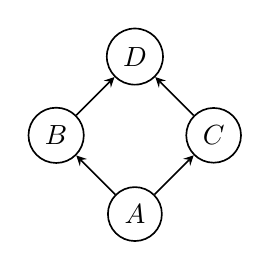
\begin{tikzpicture}[->, >=stealth, semithick]
		\tikzstyle{every node}=[draw,circle,fill=white,minimum size=4pt]
		\draw (0,0) node (A) {$A$};
		\draw (-1, 1) node (B) {$B$};
		\draw (1,1) node (C) {$C$};
		\draw (0,2) node (D) {$D$};
	
		\draw (A) -> (B);
		\draw (B) -> (D);
		\draw (A) -> (C);
		\draw (C) -> (D);
	\end{tikzpicture}
\end{figure}


%%%%%%%%%%%%%%%%%%%%%%%%%%%%%%%%%%%%%%%%%
% Hybrid Function
%%%%%%%%%%%%%%%%%%%%%%%%%%%%%%%%%%%%%%%%%
\section{Hybrid Functions}
\begin{definition}
	A \textbf{hybrid function from $\boldsymbol{S}$ to $\boldsymbol{T}$} is 
	a hybrid relation $H$ between $S$ and $T$ such that $(x,y) \in H$ and $(x,z) \in H$ implies $y=z$.
	We denote the set of all such hybrid functions by $\mathbb{Z}^{S \to T}$.
\end{definition}


Although this tells us what \emph{is} and \emph{is not} a hybrid function, it is not the most useful definition to work with. 
We would like to think of a hybrid function not as a mapping from a hybrid set to a boolean set but as
a function between two sets with a multiplicity attached to each mapping.
From this perspective, we would generally have a function and hybrid set already in mind.
Given a hybrid set $H$ over $U$ and a function $f:B \to S$ be a function where $B \subseteq U$ and $S$ a set.
Then we denote by $f^H$ the hybrid function from $B$ to $S$ defined by:
\begin{equation}
	\label{hfunc}
	f^H := \bigoplus_{x \in B} H(x) \hset{ (x, f(x) )^1 }
\end{equation}


There is little literature or established use for hybrid functions;
their primary use to us will be as something that we can turn back into traditional functions.
One may notice that we have defined hybrid functions by their graph,
taking the reduction (if it exists) of a hybrid function one naturally gets the graph of a function.


\begin{definition}
	If $H$ is a reducible hybrid set, then \textbf{$\boldsymbol{f^H}$ is a reducible hybrid function}. 
	Additionally, if $f^H$ is reducible, we extend $\mathcal{R}$ by:
	\begin{equation}
		\mathcal{R}(f^H)(x) = \restrict{f}{\mathcal{R}(H)}(x)
	\end{equation}
\end{definition}


Since $\mathcal{R}(H)$ only exists if $H(x)$ is everywhere 0 or 1; 
$\mathcal{R}(f^H)$ only makes sense when $f^H$ is reducible.
Assuming that we end up with a reducible function, hybrid functions make an excellent primitives to construct piecewise functions.
Earlier in (\ref{def:fjoin}) we defined the \emph{join of functions} to allow us to construct piecewise functions from \emph{restricted functions}.
The join of two hybrid functions is quite trivially defined.

 
\begin{definition}
	The \textbf{join}, $f^F \hjoin g^G$ of two hybrid functions $f^F$ and $g^G$ is 
	the hybrid relation given by their point-wise sum.
	\begin{equation} \label{def:hjoin}
		f^F \hjoin g^G := f^F \oplus g^G
	\end{equation}
\end{definition}


However, we will immediately dispense with using $\hjoin$ altogether and simply use $\oplus$ 
in order to prevent confusion between hybrid functional join (e.g. $f^F \oplus g^G$) and 
traditional functional join (e.g. $\restrict{f}{F} \fjoin \restrict{g}{G}$).
It is important to note that the join operator is closed under hybrid relations but not under hybrid functions.
For any two hybrid \emph{functions} the result will be a hybrid \emph{relation} 
but not necessarily another hybrid function.
As with traditional functional join, we must still be wary of overlapping regions
 but non-disjoint hybrid domains are not nearly as ``dangerous''.
For intersecting regions we do not have to choose between commutivity and associativity, we can have both.
In general, all that we can say the result is a hybrid relation but there are many cases where we can guarantee hybrid function status is preserved.


\begin{theorem}
Let $A$ and $B$ be hybrid sets over $U$ and let $f: U \to S$ be a function.
Then $f^A \oplus f^B$ is a hybrid function.
Moreover,
	\begin{equation}
		f^A \oplus f^B = f^{A \oplus B}
	\end{equation}
\end{theorem}


It should not be a surprise that the same function over different restrictions combine to form a function.
Let $(x,f(x)) \in f^A$ and $(y,f(y)) \in B$. Clearly, if $x=y$ then $f(x)=f(y)$. 
Since $f$ is common between both hybrid functions, there cannot be disagreement among points.
Additionally,
\begin{align}
	f^A \oplus f^B 
		&= \bigoplus_{x \in U} A(x) \hset{ (x, f(x) )^1 } 
			\; \oplus \; \bigoplus_{x \in U} B(x) \hset{ (x, f(x) )^1 } \notag \\
		&= \bigoplus_{x \in U} (A(x) + B(x)) \hset{ (x, f(x) )^1 } \notag \\
		&= \bigoplus_{x \in U} (A \oplus B)(x) \hset{ (x, f(x) )^1 }
\end{align}


Inductively, this holds for any number of hybrid sets with a common function.
For instance, given any generalized partition $P = P_1 \oplus P_2 \oplus \ldots \oplus P_n$, 
we have the following equation reminiscent of (\ref{fjoin_partition}):
\begin{equation}
 	f^P = f^{P_1} \oplus f^{P_2} \oplus \ldots \oplus f^{P_n}
\end{equation}


Joining a function with itself is not the most interesting construction.
Piecewise functions are useful for their ability to tie together two \emph{different} functions.
If two functions have separate, non-overlapping regions, then our definition is again trivial.


\begin{theorem}
	Given two function $f : U \to S$ and $g : U \to S$. The following identity holds if and only if $A$ and $B$ are disjoint:
	\begin{equation}
		f^A \oplus g^B = (f \fjoin g)^{A \oplus B}
	\end{equation}
\end{theorem}


Notice here the use of $\fjoin$ on the right hand side.
Here $\fjoin$ is traditional (non-hybrid) function join.
Since $A$ and $B$ are disjoint, the problems that arose earlier are not an issue.
In fact, it doesn't even matter which convention we use.
Disjointness is still too strong of a condition for two hybrid functions to be compatible.
The join of two non-disjoint functions may still be a hybrid function 
even if their respective functions do not agree at \emph{all} points.
So long as long as they agree on all points in overlapping regions intersection the functions can be safely joined.


\begin{definition}
	For hybrid functions $f^A$ and $g^B$, $f^A \oplus g^B$ is a hybrid function
	if and only if for all $x \in \text{supp} (A \otimes B)$, we have $f(x) = g(x)$.
	We say that \textbf{$\boldsymbol{f^A}$ and $\boldsymbol{g^B}$ are compatible}.
\end{definition}


As with our definition of disjointness, we use the pointwise product $\otimes$ 
of hybrid sets as an analog for intersection $\cap$ of sets.
This definition also generalizes the two cases we have already seen in theorems 2.3.1 and 2.3.2.
The hybrid functions $f^A$ and $f^B$ are clearly compatible because $f$ agrees with itself everywhere.
For $A$ and $B$ disjoint, $f^A$ and $g^B$ are also compatible since $A \otimes B$ is empty;
there are no mutual points for $f$ and $g$ to disagree over.

Compatibility becomes less clear when we begin to consider multiple hybrid functions.
For one, compatibility is not associative.
Consider the following sequence:


\begin{equation}
(f^H \oplus g^H) \oplus g^{\ominus H} = f^H \oplus (g^H \oplus g^{\ominus H}) = f^H \oplus g^\emptyset = f^H
\end{equation}

$g^H$ and $g^{\ominus H}$ are clearly compatible by 2.3.1.
The resulting $g^{\emptyset}$ is compatible with \emph{any} hybrid function.
Although $f^H$ and $g^H$ could be mutually incompatible; 
we can only certain that $f^H \oplus g^H$ is a hybrid relation.
Regardless of their compatibility, when this is joined with $g^{\ominus H}$, the $g$ terms cancel
and we are left with \emph{is} a hybrid function.





%%%%%%%%%%%%%%%%%%%%%%%%%%%%%%%%%%%%%%%%%
% *-Reducible
%%%%%%%%%%%%%%%%%%%%%%%%%%%%%%%%%%%%%%%%%
\section{Hybrid Function Fold}


Compatibility and reducibility are one way of collapsing a hybrid function to a traditional function.
Another approach is to fold or aggregate a hybrid function using some operator.
To aid in this we will first introduce some notation for iterated operators.
\begin{definition}
	Let $\op : S \times S \to S$ be an operator on $S$.
	Then, for $n > 0$, $n \in \mathbb{Z}$ we use $\op^n:S \times S \to S$ to denote iterated $\op$.
	So,
	\begin{equation}
		x \op^n y = (((x \overbrace{\op y) \op y) \op \ldots \op y)}^{n \text{ times}}
	\end{equation}
	If $\op$ has an identity $e_\op$, then we extend $x \op^0 y = x$.
	If $\op$ is invertible, then we use $\op^{-1}$ to denote its inverse and $\op^{-n}$ for iterated $\op^{-1}$.
	Finally, we allow $\op^n$ to be a unary operator, which we define by $\op^n x = e_\op \op^n x$.
\end{definition}

Assuming $\op^m$ and $\op^n$ are both defined (e.g. if $m,n \leq 0$ then $\op$ must be invertible),
we have $ ( x \op^m y ) \op^n y = x \op^{m+n} y$.

For non-associative magmas, it may be of interest to instead define $\op^T$ for some tree $T$. 
For example $\op^n$ above is analogous to Haskell's \texttt{foldl}.
There are applications where \texttt{foldr}: $(x \op ( y \op ( y \op \ldots \op y)))$ or a balanced expression tree like \texttt{foldt} might be desired.
Most applications however will be interested in group operators and so we will not explore this.

\begin{definition}
	We say that a hybrid relation $f^A = f_1^{A_1} \oplus f_2^{A_2} \oplus \ldots$ over $T \times S$ 
	is $\op$\textbf{-reducible} if $(S, \op)$ is an abelian group 
	or if $(S, \op)$ is an abelian semi-group and $f^A$ is everywhere non-negative.
	If $f^A$ is $\op$-reducible we define its $\op$\textbf{-reduction}, $\mathcal{R}_\op(f^A) :  T \to S$ 
	as a (non-hybrid) function given by:
	\begin{equation}
		\mathcal{R}_\op (f^A)(x) = \restrict{\left(\op^{A_1(x)} f_1(x) \op^{A_2(x)} f_2(x) \op \ldots \right)}{\supp A}
	\end{equation}
\end{definition}


If $f^A$ is reducible then it is trivially $\op$-reducible and we have:
\begin{equation}
	\mathcal{R}(f^A) = \mathcal{R}_\op(f^A)
\end{equation}
If a hybrid function is already ``flattened'', then reducing it will do nothing.
So clearly $\mathcal{R}_\op$ is a projection since it is idempotent  (i.e. $\mathcal{R}_\op ( \mathcal{R}_\op( f^A)) = \mathcal{R}_\op(f^A)$).
Moreover,
\begin{equation}
	\mathcal{R}_\op( \mathcal{R}_\op(f^F) \oplus \mathcal{R}_\op(g^G)) =\mathcal{R}_\op( f^F \oplus g^G)
\end{equation}

\todo[inline]{$\mathcal{R}_\times ( \mathcal{R}_+ \oplus \mathcal{R}_+ )$}

\subsection{Example: \emph{Sign function}}

One would typically write the sign function out as a piecewise function over 3 regions of the extended real line: 
$(-\infty, 0)$, $\{ 0 \}$, and $(0, \infty)$.
Or alternatively using a $+$-reduction using 2 pieces: $(-\infty, 0]$ and $[0, \infty)$.
\begin{equation}
	\text{sign} \;=\; -1^{(-\infty, 0)} \hjoin 0^{\{0\}} \hjoin 1^{(0, \infty)}
	\;=\; \mathcal{R}_+ \left( -1^{(-\infty, 0]} \oplus 1^{[0, \infty)} \right)
\end{equation}
Evaluation of the $\text{sign}$ at the points 1 or 0 is performed as follows:
\begin{equation*}
 \text{sign}(1) = \mathcal{R}_+ \left( -1^{(-\infty, 0]} \oplus 1^{[0, \infty)} \right)(1) 
 = \mathcal{R}_+ \left( -1^{0} \oplus 1^{1} \right)
 = +^0 (-1) +^1 (1) = 1
\end{equation*}
\begin{equation*}
 \text{sign}(0) = \mathcal{R}_+ \left( -1^{(-\infty, 0]} \oplus 1^{[0, \infty)} \right)(0) 
 = \mathcal{R}_+ \left( -1^{1} \oplus 1^{1} \right)
 = +^1 (-1) +^1 (1) = 0
\end{equation*}

Going from 3 regions to 2 may seem a small step.
However, consider two piecewise functions with $n$ and $m$ regions respectively.
Taking the sum of these two functions would lead to a new piecewise function with $n\cdot m$ regions.
We will show that $\op$-reductions can allow us to reduce this to only a linear increase!


%%%%%%%%%%%%%%%%%%%%%%%%%%%%%%%%%%%%%%%%%
% Piecewise 1
%%%%%%%%%%%%%%%%%%%%%%%%%%%%%%%%%%%%%%%%%
\subsection{Example: \emph{Piecewise functions on generalized partitions}} 
Let $A_1 = [0,a)$, $A_2 = [0,1] \setminus A_1$, $B_1 = [0,b)$ and $B_2 = [0,1] \setminus B_1$.
As well as piecewise functions $f$ and $g$ given as:
\begin{equation*}
	f(x) = f_1^{A_1} \oplus f_2^{A_2}
		= \begin{cases}
			f_1(x) & x \in A_1 \\
			f_2(x) & x \in A_2
		\end{cases}
	\;\;\;\;\; \text{and} \;\;\;\;\;
	g(x) = g_1^{B_1} \oplus g_2^{B_2}
		= \begin{cases}
			g_1(x) & x \in B_1 \\
			g_2(x) & x \in B_2
		\end{cases}
\end{equation*}

If one were interested in computing the piecewise function $(f+g)$, the na\''{i}ve method would be to take the pairwise
sum of each sub-function. 
Then restrict each sum to the intersection of respective partitions as below:
\begin{equation}
	(f+g)(x) = (f_1 + g_1)^{A_1 \cap B_1} 
		\oplus (f_1 + g_2)^{A_1 \cap B_2} 
		\oplus (f_2 + g_1)^{A_2 \cap B_1}
		\oplus (f_2 + g_2)^{A_2 \cap B_2}
\end{equation}

We will take another approach.
First, we can partition $[0,1]$ into the generalized partition $A_1$, $B_1 \ominus A_1$, $B_2$.
The source of this particular partition will remain mysterious for now but observe that we can still construct the partitions:
$B_1 = (B_1 \ominus A_1) \oplus A_1$ and $A_2 = (B_1 \ominus A_1) \oplus B_2$.
And so we can represent $f$ and $g$ from above with a common partition by using:
\begin{align}
	f &=  f_1^{A_1} \;\oplus\; f_2^{(B_1 \ominus A_1) \oplus B_2}
		\;=\; f_1^{A_1} \;\oplus\; f_2^{B_1 \ominus A_1} \;\oplus\; f_2^{B_2} \\
	g &= g_1^{A_1 \oplus (B_1 \;\ominus\; A_1)} \;\oplus\; g_2^{B_2}
		\;=\; g_1^{A_1} \;\oplus\; g_1^{B_1 \;\ominus\; A_1} \;\oplus\; g_2^{B_2}
\end{align}

Since we have a common partition we can avoid computing pairwise intersections altogether and simply add each 
sub-function to the corresponding sub-function which shares a partition.
Since $\{ A_1 , B_1, (B_1 \ominus A_1) \}$ is a generalized partition, we will need to flatten the expression back down
to get a traditional function.
We use $\mathcal{R}_+$ for this so that negative regions properly cancel. 

\begin{equation}
	(f+g)(x) = \mathcal{R}_+ \left( (f_1 + g_1)^{A_1} 
			\oplus (f_2 + g_1)^{B_1 \ominus A_1} 
			\oplus (f_2 + g_2)^{B_2} \right)
\end{equation}


This equation holds regardless of the relative ordering of $a$ and $b$.
Suppose $x \in A_1 \cap B_1$
Then we have $A_1(x)= 1$ and $(B_1 \ominus A_1)(x) = B_2(x) = 0$.
And so $(f+g)(x) = (f_1 + g_1)(x)$.
Similarly, if $x \in B_1 \cap A_2$ or $x \in A_2 \cap B_2$ then 
only $(B_1 \ominus A_1)(x)$ or $B_2(x)$ will respectively be non-zero.
However, if $x \in B_2 \cap A_1$ then we have $A_1(x) = 1$, $(B_1 \ominus A_1)(x) = -1$ and $B_2(x) = 1$.
Simplifying this expression yields:
\begin{equation}
	(f+g) \;=\; +^1 (f_1 + g_1) +^{-1} (f_2 + g_1) +^1 (f_2 + g_2) \;=\; (f_1 + g_2)
\end{equation}


%%%%%%%%%%%%%%%%%%%%%%%%%%%%%%%%%%%%%%%%%
% Refinement
%%%%%%%%%%%%%%%%%%%%%%%%%%%%%%%%%%%%%%%%%
In the above example only three regions could simultaneously exist.
If $a<b$ then $A_1 \cap B_2 = \emptyset$ but if $b<a$ then $A_2 \cap B_1 = \emptyset$.
Although it might seem that the three terms are a result of three regions, in the general case where 
$A_1$ and $B_1$ could be arbitrary subsets, we still only have three terms.
We will even extend this to any generalized partition.
First we will formalize some ideas we have already seen.


\begin{definition}
	A \textbf{refinement} of a generalized partition $P = \{P_i\}_{i \in I}$ is another generalized partition
	$Q = \{Q_j \}_{j \in J}$ such that, for every $P_i$ in $P$ there is a subset of $Q$: $\{ Q_{j} \}_{j \in J_i}$, 
	$J_i \subseteq J$ such that for some integers $\{a_{i,j}\}_{j \in J_i}$
	\begin{equation}
		P_i = \bigoplus_{j \in J_i} a_i,j Q_{j}
	\end{equation}
	Given a \emph{set} of generalized partitions a \textbf{common refinement} is a generalized partition which is a 
	refinement of every partition in the set. 
	A refinement $Q$ of $P$ is \textbf{strict} if $\text{supp}(Q) = \text{supp}(P)$.
\end{definition}


In our previous example we used $\{ A_1, B_1 \ominus A_1, B_2 \}$ which was a common refinement of both
$\{ A_1, A_2 \}$ and $\{ B_1, B_2 \}$.
$A_1$ and $B_2$ have trivial representations while $A_2 = (B_1 \ominus A_1) \oplus B_2$ and 
$B_1 = A_1 \oplus (B_1 \ominus A_1)$.
Another common refinement would be the trivial $\{ A_1, B_1, A_2, B_2 \}$
This is less preferable due to not only containing 4 regions instead of 3 but also the pointwise sum is $[0,1]^2$
instead of the reducible $[0,1]$.

We can now formally phrase our problem.
Let $A=\{ A_i \}_{i \in [n]}$ and $B=\{ B_j \}_{j \in [m]}$ be two generalized partitions of a hybrid set $U$ 
(where $[n] = \{ 1, \ldots, n \}$ for $n \in \mathbb{N}$).
We wish to find a generalized partition $C$  of $U$ which is a \emph{common}, \emph{strict} refinement of $A$ and $B$
and has minimal cardinality.
These conditions can be summarized into the following linear system of $n+m+1$ simultaneous equations:
\begin{equation}
	U = \bigoplus_i C_i
\end{equation}
\begin{equation}
	\forall i \in [n] : A_i = \bigoplus_j  a_{i,j} C_j
\end{equation}
\begin{equation}
	\forall j \in [m] : B_j = \bigoplus_i b_{i,j} C_i
\end{equation}
for some integers $a_{i,j}$ and $b_{i,j}$.
Since we know that $A$ and $B$ are each partitions of $U$, only $n+m-1$ can be independent.
If there are additional dependencies betwen $A$ and $B$ then this can be even lower.
Expressed as a linear system we have:


\begin{equation}
	M \cdot 
		\begin{pmatrix}
			C_1 	\\
			\vdots 	\\
			C_{n+m-1}
		\end{pmatrix}
	=
		\begin{pmatrix}
			U 		\\[-0.5em] 
			A_1 	\\[-0.5em] 
			\vdots 	\\[-0.5em] 
			A_{n-1}	\\[-0.5em] 
			B_1 	\\[-0.5em] 
			\vdots 	\\[-0.5em] 
			B_{m-1}
		\end{pmatrix}
	\;\;\;\;\;\;\text{ where }\;\;
	M = \begin{pmatrix}
			1			& 1			& \cdots 	& 1 					\\[-0.5em]
			a_{1,1}		& a_{1,2}	& \cdots 	& a_{1, n+m-1} 		\\[-0.5em]
			\vdots 		&			&			& \vdots 			\\[-0.5em]
			a_{n-1,1}	& a_{n-1, 2}	& \cdots 	& a_{n-1, n+m-1} 	\\[-0.5em]
			b_{1,1} 		& b_{1,2} 	& \cdots 	& b_{1, n+m-1}		\\[-0.5em]
			\vdots 		& 			&			& \vdots 			\\[-0.5em]
			b_{m-1,1} 	& b_{m-1,2}	& \cdots 	& b_{m-1,n+m-1}
	\end{pmatrix}
\end{equation}


By definition, $M$ is an integer matrix.
But we are actually more interested in its inverse $M^{-1}$ as this will give us values for $C_i$ 
relative to $( U, A_1, \ldots, A_{m-1}, B_1, \ldots, B_{m-1} )$.
To stay in the realm of hybrid sets, we would also like to enforce that $M^{-1}$ is also an integer matrix.
Assuming this, then the determinant of $M$ must be $\pm 1$.
Further restricting ourselves to upper triangular matrices we can choose $M$ to be all 1's along the diagonal
as well as the top row. 
Which has the following inverse:
\begin{equation}
	\begin{pmatrix}
		1 		&\cdots 	&\cdots 	&\cdots 	& 1 		\\[-0.5em]
		0		& 1		& 0 		&\cdots 	& 0 		\\[-0.5em]
		\vdots 	&\ddots 	&\ddots 	&\ddots 	&\vdots 	\\[-0.5em]
		\vdots 	&		&\ddots 	&\ddots 	& 0 		\\[-0.5em]
		0 		&\cdots 	&\cdots 	& 0 		& 1
	\end{pmatrix}^{-1}
	= \; \; \;
	\begin{pmatrix}
		1 		&-1	 	&\cdots 	&\cdots 	& -1		\\[-0.5em]
		0		& 1		& 0 		&\cdots 	& 0 		\\[-0.5em]
		\vdots 	&\ddots 	&\ddots 	&\ddots 	&\vdots 	\\[-0.5em]
		\vdots 	&		&\ddots 	&\ddots 	& 0 		\\[-0.5em]
		0 		&\cdots 	&\cdots 	& 0 		& 1
	\end{pmatrix}
\end{equation}



Thus we find that for the partitions $A = \{ A_i \}_{i \in [n]}$ and $B = \{ B_j \}_{j \in [m]}$ we can \emph{always}
use the strict, common and minimal refinement:
\begin{equation}
	\Big\{ (U \ominus A_1 \ominus \ldots \ominus A_{n-1} \ominus B_1 \ominus \ldots \ominus B_{n-1}), \;\;
	A_1, A_2, \ldots, A_{n-1}, \;\; B_1, B_2, \ldots, B_{m-1}
	\Big\}
\end{equation}
Finally, to generalize our example from earlier, let $f = f_1^{P_1} \oplus f_2^{P_2} \oplus f_n^{P_n}$
and  $g = g_1^{Q_1} \oplus \ldots \oplus g_m^{Q_m}$ be two piecewise functions over a common domain $U$.
We can compute $f \op g$ by:
\begin{align}
f \op g = \; \mathcal{R}_\op  \; & \!\!\! \left( \,
		(f_1 \op g_m)^{P_1} 
		\oplus \ldots \oplus 
		 (f_{n-1} \op g_m)^{P_{n-1}} \right. \notag \\
	\oplus & \;
		 (f_n \op g_1)^{Q_1} 
		\oplus \ldots \oplus 
		 (f_n \op g_{m-1})^{Q_{m-1}} \notag \\
	\oplus & \left. 
		 (f_n \op g_n)^{U \ominus (P_1 \oplus \ldots \oplus Q_{n-1} \oplus Q_1 \oplus \ldots \oplus Q_{m-1})}
	\; \right)
\end{align}


This is not a unique formulation.
Any upper triangular matrix containing only 1, 0 and $-1$ and all 1's in the first row would also be acceptable.
Each would lead to slightly different forms of (2.47). This particular choice is merely one of the simplest options. 
Certain applications could lead to other choices of $M$ for reasons of memory efficiency, but it is not clear this is needed.

%%%%%%%%%%%%%%%%%%%%%%%%%%%%%%%%%%%%%%%%%
%
% PSEUDO-FUNCTIONS
%
%%%%%%%%%%%%%%%%%%%%%%%%%%%%%%%%%%%%%%%%%
\section{Pseudo-functions}

One last detail remains to be settled, the sub-functions $f_i$ and $g_j$ may not be defined outside of 
$P_i$ and $Q_j$ respectively.
Consider the equation in (2.47), evaluated at $x \in P_1 \cap Q_1$.
Then we have the following terms with non-zero multiplicity.
\begin{equation}
	(f \op g)(x) = \mathcal{R}_\op 
		\left(   (f_1(x) \op g_m(x))^1 \oplus 
				(f_n(x) \op g_1(x))^1 \oplus 
				(f_n(x) \op g_m(x))^{-1} 
		\right)
\end{equation}


We would like for the $g_m(x)$ in the first term to cancel with the $g_m(x)$ in the third.
If $q_m$ (and $f_n$) are defined and finite at all points in $U$, then there is no problem.
However if $g_m(x)=\infty$, then we need to make cumbersome arguments for: $ \infty + y - \infty = y$.
To resolve this, we use a lambda-lifting trick to have a hybrid relation over the domain and \emph{the function itself}
rather than the domain and the image implied by the function.


\begin{definition}
	Using the same notation as in our definition from (\ref{hfunc}), we define a pseudo-function $\tilde{f}^A$ as:
	\begin{equation}
 		\tilde{f}^A = \bigoplus_{x \in B} A(x) \hset{(x,f)^1}
	\end{equation}
\end{definition}


One should notice the similarity between (2.49) and (2.22).
The difference is that we have replaced $(x, f(x))$ with the unevaluated $(x,f)$.
This formally makes $\tilde{f}^A$ a hybrid relation over $U \times (U \to S)$ as opposed to 
a hybrid function over $U \times S$.
To evaluate $\tilde{f}^A$ we map back to $f^A$ and evaluate that.
This mapping between $(x,f(x))$ and $(x,f)$ is very natural and we will perform it unceremoniously,
often using $f^A$ and $\tilde{f}^A$ interchangeably. 
Properties of hybrid functions such as compatibility and reducibility will be lifted to hybrid pseudo-functions by this as well.


%%%%%%%%%%%%%%%%%%%%%%%%%%%%%%%%%%%%%%%%%
% Piecewise 2
%%%%%%%%%%%%%%%%%%%%%%%%%%%%%%%%%%%%%%%%%
\subsection{Example: \emph{Piecewise functions revisited}}


We will repeat the example from 2.4.2 but concretely using the following function:
\begin{equation}
	f(x) = \begin{cases}
		(2-x^2) & -1 \leq x \leq 1\\
		1/x^2 & \text{otherwise}
	\end{cases}
\end{equation}
Graphically, this is a mundane-looking bell-shaped curve shown in black in Figure 2.2.
Although $f$ is defined for all of $\mathbb{R}$, this is not the case for its sub-functions. 
The plots in red and blue show the behaviour of $(2-x^2)$ and $1/x^2$ outside of their defined ranges in $f$.


\begin{figure}[h]
	\caption[Piece-wise Rational Function]{A piecewise rational function is shown in black. 
	The plots in red and blue are continuations of $(2-x^2)$ and $1/x^2$ respectively.
	\label{fig:pwRational}}
	\centering
	\begin{tikzpicture}[>=stealth]
	    \begin{axis}[
	        xmin=-5,xmax=5,
	        ymin=-2,ymax=10,
	        axis x line=middle,
	        axis y line=middle,
	        axis line style=<->,
	        xlabel={$x$},
	        ylabel={$y$},
	        ]
	        \addplot[no marks,black,thick,-] expression[domain=-1:1,samples=100]{2 - x^2};
	        \addplot[no marks,blue,->] expression[domain=-1:-0.33,samples=100]{1/x^2};
	        \addplot[no marks,blue,<-] expression[domain=0.33:1,samples=100]{1/x^2};
	        \addplot[no marks,black,thick,<-] expression[domain=-4:-1,samples=100]{1/x^2};
	        \addplot[no marks,red,<-] expression[domain=-2:-1,samples=100]{2 - x^2};
	        \addplot[no marks,black,thick,->] expression[domain=1:4,samples=100]{1/x^2};
	        \addplot[no marks,red,->] expression[domain=1:2,samples=100]{2 - x^2};
	    \end{axis}
	\end{tikzpicture}
\end{figure}


Represented as a hybrid pseudo-functions we have $\tilde{f}$ as:

\begin{equation}
	\tilde{f} = \tilde{f_1}^{A_1} \oplus \tilde{f_2}^{A_2} 
	  = (x \mapsto 2-x^2)^{[-1, 1]} \oplus (x \mapsto 1/x^2)^{(-\infty, -1) \oplus (1, \infty)}
\end{equation}
which we are interested in multiplying by the unevaluated absolute value function:
\begin{equation}
	\tilde{g} = \tilde{\text{abs}} = (x \mapsto x)^{[0, \infty )} \oplus (x \mapsto -x)^{(-\infty, 0)}
\end{equation}

First we must find a minimal common refinement.
Using the formula in (2.46), we decide to use the partition:
\begin{align}
	P_1 &= [-1,1] \\
	P_2 &= [0, \infty) \\
	P_3 &= \mathbb{R} \ominus [-1,1] \ominus [0, \infty)
\end{align}
where $P_3$ could also be simplified into disjoint regions by $P_3 = (-\infty, -1) \ominus [0,1]$.
Thus we have the expression
\begin{align}
	(\tilde{f} \times \tilde{g}) = \mathcal{R}_\times \bigg(
				& \left( (x \mapsto 2-x^2) \times (x \mapsto -x) \right)^{P_1} \notag \\
		\oplus \;& \left( (x \mapsto 1/x^2) \times (x \mapsto -x) \right)^{P_2} \notag \\
		\oplus \;& \left( (x \mapsto 1/x^2) \times (x \mapsto -x) \right)^{P_3} 
	\bigg)
\end{align}
If we use pseudo-functions then we assign multiplicities to the still unevaluated sub-functions.
So, for example to evaluate $(f \times g)$ at 0, we would evaluate each of $P_1$, $P_2$ and $P_3$ at 0 and find:
\begin{align}
	(\tilde{f} \times \tilde{g})(0) = \mathcal{R}_\times \bigg(
				& \left( (x \mapsto 2-x^2) \times (x \mapsto -x) \right)^1 \notag \\
		\oplus \;& \left( (x \mapsto 1/x^2) \times (x \mapsto -x) \right)^1 \notag \\
		\oplus \;& \left( (x \mapsto 1/x^2) \times (x \mapsto -x) \right)^{-1} 
	\bigg)(0)
\end{align}
Once we have this, we can then evaluate the $\times$-reduction on the still unevaluated functions.
Clearly $x \mapsto -x$ occurs with cancelling signs as does $x \mapsto 1/x^2$.
This leaves us with the product of two unevaluated functions:
\begin{equation}
	(\tilde{f} \times \tilde{g})(0) = \left((x \mapsto 2-x^2) \times (x \mapsto x)\right) (0)
\end{equation}


\emph{After} these cancellations occur, then it is finally safe to evaluate at a point and 
we find $(\tilde{f} \times \tilde{g})(0)=0$ as expected.
To contrast this, if one were to attempt to evaluate a the (non-pseudo) hybrid function version of 
$\tilde{f} \times \tilde{g}$, instead of (2.57) one would have the expression:
\begin{equation}
	(f \times g)(0) = \mathcal{R}_\times \left( (2 \times 0)^1 \oplus (\text{``}\infty\text{''} \cdot 0)^1 \oplus (\text{``}\infty\text{''} \cdot 0)^{-1} \right)
\end{equation}
Simplifying the $\times$-reduction leads to both $\infty / \infty$ and $0/0$.
Although they \emph{should} obviously cancel, the behaviour is not well defined.














\newpage